\section{Vs in big data}\label{Vs}
Vs in big data represent challenges we are going to encounter. There are 3 main Vs (volume, variety and velocity) that are seen on the image bellow \parencite{sagiroglu2013big}. Over the years, new challenges have occurred with data therefore new Vs have been added \parencite{anuradha2015brief}. 

Described bellow are main 3 Vs with 2 additional ones.

\begin{figure}[H]
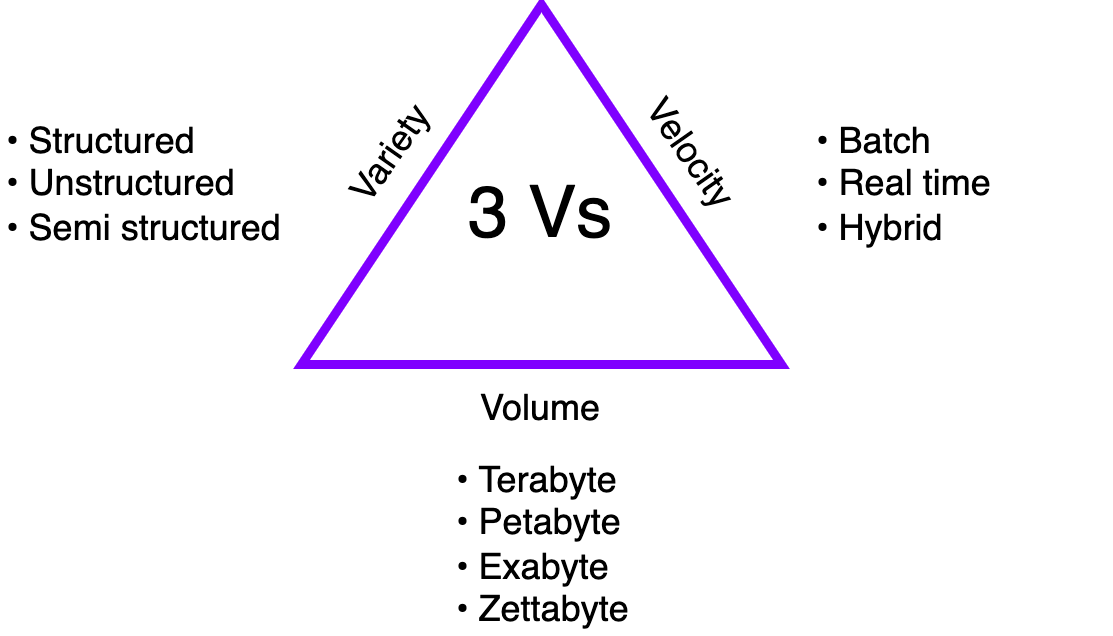
\includegraphics[scale=0.25]{img/Vs/BigData-Vs.png}
\centering
\caption{Vs}
\label{fig:Vs}
\end{figure}

%Source: https://ieeexplore.ieee.org/abstract/document/6567202/figures#figures
%Doug defined 3vs  https://scholar.google.co.uk/scholar?hl=en&as_sdt=0%2C5&as_vis=1&q=Big+Data+Computing+Using+Cloud-Based+Technologies%3A+challenges+and+opportunities&btnG=&oq=Big+Data+Computing+Using+Cloud-Based+Technologies%3A+Challenges+and

%Source: https://link.springer.com/chapter/10.1007/978-3-319-06811-4_13
\newpage
\subsection{Volume}\label{Volume}

Volume is a representation of data coming into the computer (server). It is measured in computer storage capacity \parencite{katal2013big}. 

In our case, we have data at rest (it will not change). The total storage equals to:

\begin{table}[h]
\centering
\begin{tabular}{|l|r|}
\hline
\text{file name} & \text{size} \\
\hline
\text{chat\_join\_team\_chat.csv} & 82 \, \text{KB} \\
\text{chat\_leave\_team\_chat.csv} & 67 \, \text{KB} \\
\text{chat\_mention\_team\_chat.csv} & 238 \, \text{KB} \\
\text{chat\_respond\_team\_chat.csv} & 252 \, \text{KB} \\
\text{combined-data.csv} & 162 \, \text{KB} \\
\text{ad-clicks.csv} & 826 \, \text{KB} \\
\text{buy-clicks.csv} & 135 \, \text{KB} \\
\text{game-clicks.csv} & 33.8 \, \text{MB} \\
\text{level-events.csv} & 43 \, \text{KB} \\
\text{team-assignments.csv} & 331 \, \text{KB} \\
\text{team.csv} & 8 \, \text{KB} \\
\text{user-session.csv} & 492 \, \text{KB} \\
\text{users.csv} & 137 \, \text{KB} \\
\hline
\text{Total file size} & \text{36.436 MB} \\
\hline
\end{tabular}
\caption{Files and Sizes}
\label{FileSizes}
\end{table}

In total we are dealing with 36.436 MB (or 36436 KB). This can work as a representation of big data, but in reality we would be dealing with more sophisticated files (bigger file sizes, more file types, more files, etc...)

\subsection{Variety}\label{Variety}

Variety describes the kind of data we are dealing with. This can be from text, to video, sound, etc... Different files carry different burdens, for example file size. Video platform (such as YouTube) is distributing mainly video formats \parencite{hota2018big}, therefore they need a different infrastructure compared to text based website (such as Stack overflow).

As seen in table above (\ref{FileSizes}), we are mainly dealing with CSV files. This is represented in semi structured form since we can link items together. In the processing stage, files could be change to different format in order to save space (example: Parquett with Apache Hudi).
\subsection{Velocity}\label{Velocity}

Velocity represents frequency of data ingestion. How often we receive data depends on the system we are talking about \parencite{cappa2021big}. It can be once a second (video stream), every hour (record update), every 6 moths, etc... Frequency is important from computational point of view. If we only expect data every week, data pipeline will need to be executed one a week, otherwise if data is received every second, our pipeline needs to be running all the time (24/7).

In our case, we have already received data beforehand. That means we have data at rest, we are not expecting it to change. In case we would have access to live data (with an API for example), our records would be changing based on each run.
\subsection{Veracity}\label{Veracity}
Veracity represents how data is accurate, reliable and certain. To accomplish this, we can use different approaches \parencite{rubin2013veracity}. If data is stored at one storage medium (SSD/HDD/USB) and that gets damaged, we could experience data loss. The best practise is to use 3-2-1 approach \parencite{storage2012data}:
\begin{itemize}
    \item 3 copies of data
    \item 2 different media
    \item 1 copy being off-site
\end{itemize}
This can be achieved by using one of the cloud providers (AWS, Azure, Google Cloud, etc...) in order to save data across the word.

To insure quality, we would need to restrain data either at input level or at processing. If we have complete access to the data based on its life cycle, we can impose rules at the beginning of insertion (limit age, countries available, etc...) \parencite{yu2010view}. Otherwise if we don't have access to data from the start, we can apply rules in the data processing stage.

In our case, we don't need to worry about the data loss since data is hosted on GitHub \parencite{web:GitHub}. By using cloud service to host our data we don't need to worry about 3-2-1 since they are taking care of it \parencite{wang2010toward}. There are also historical versions of our files available which is beneficial. Disadvantage is that we don't control the infrastructure, meaning if GitHub (owned by Microsoft) would disappear overnight, all of the data is gone.

In order to assure data quality, we are doing data transformations in the processing stage. One example is date time. In some of the files it is saved as YYYY-mm-DD HH:MM:SS while in others it is in Unix time format. Due to benefits of Unix time (deeper dive at \ref{A0}), all the time was converted to it. If we would have control from the beginning, small bugs like this could have been fixed at source.
\subsection{Value}\label{Value}

Value provides business insights of the data. This can be interpreted in a number of ways, such as most of the players are from US therefore lets focus our infrastructure there, a lot of players seem to click on technology related ads lets expand that, etc....

Data can provide different value to the company. It all depends on context and analysts extracting it.

In our case, the biggest value it provides is players. With it we can see where they are from, age, platform, etc... Chat data is available as well but it doesn't provide as much details for us but for players it is a lot more important since they can communicate between each other.
Value can also be added from external sources. For example, we have Twitter handles in our data. We could expand our dataset by doing text mining on each users Twitter profile in order to server them personalised advertisements. This would increase our data value and financial gain as a company.

